\documentclass[letterpaper]{article}
\usepackage{amssymb}
\usepackage{fullpage}
\usepackage{changepage}
\usepackage{amsmath}
\usepackage{epsfig,float,alltt}
\usepackage{psfrag,xr}
\usepackage[T1]{fontenc}
\usepackage{url}
\usepackage{pdfpages}
\usepackage{epstopdf}
\usepackage[framed,numbered,autolinebreaks,useliterate]{mcode}

%\includepdfset{pagecommand=\thispagestyle{fancy}}
\author{Yi Yang}
\title{EECS 442 Homework \#4}

\begin{document}
\date{11/25/2016}
\maketitle

\newcommand{\trace}{\mathrm{trace}}
\newcommand{\real}{\mathbb R}  % real numbers  {I\!\!R}
\newcommand{\nat}{\mathbb N}   % Natural numbers {I\!\!N}
\newcommand{\cp}{\mathbb C}    % complex numbers  {I\!\!\!\!C}
\newcommand{\ds}{\displaystyle}
\newcommand{\mf}[2]{\frac{\ds #1}{\ds #2}}
\newcommand{\spanof}[1]{\textrm{span} \{ #1 \}}
\newcommand{\sol}[0]{\textbf{Solution: }}
\newcommand{\pf}[0]{\textbf{Proof:}}
\newcommand{\rme}[0]{\textrm{e}}
\newcommand{\Null}[1]{\textrm{Null}\{#1\}}
\parindent 0pt
%%%%%%%%%%%%%%%%%%%%%%%%%%%%%%%%%%%%%%%%%%%%%%%%%%%%%%%%%%%%%%%%%%%%%%%%%%%%%%%
% Solution for Question 1 begins here - by Yi Yang
%%%%%%%%%%%%%%%%%%%%%%%%%%%%%%%%%%%%%%%%%%%%%%%%%%%%%%%%%%%%%%%%%%%%%%%%%%%%%%%
\section*{Problem 1 \underline{Harris Corner Detection}}
\subsection*{(a)}
Steps for Harris Corner Detection:
\begin{itemize}
	\item Compute partial derivatives at each pixel
	\item Compute second moment matrix M in a Gaussian window around each pixel
	\item Compute corner response function R
	\item Threshold R
	\item Find local maxima of response function (nonmaximum suppression)
\end{itemize}
The size we chose for the Gaussian window is $w = 3$. Note that in the codes we use Sobel filter as the derivative filter as the approximation of gradient at each pixel, other derivative filters include Prewitt filter or Robert filter. By applying derivative filter, we can easily calculate the second moment matrix at each pixel. The methods using ellipses and corner response function are both coded and Matlab function $ELLIPSE()$ is used to plot ellipses in the original figures.
\lstinputlisting[firstline=1, lastline=200]{q1solution.m}
\lstinputlisting[firstline=1, lastline=200]{ellipse.m}

\clearpage

\subsection*{(b)}
The Gaussian window size I chose are $w = 3$, $w = 4$, $w = 7$ and $w = 10$, the results for image $I1$ and $I3$ are listed below. From results shown in Fig. \ref{I1w3}$\sim$ \ref{I1w10} and Fig. \ref{I3w3}$\sim$ \ref{I3w10}, we find that the ellipses are easily distinguished and the corner detection is highly effective. However, as we increase the window size, the ellipses gradually become hard to be distinguished from its environment, the effects of detector become worse as window size increases.
\begin{figure}[H]
\centering
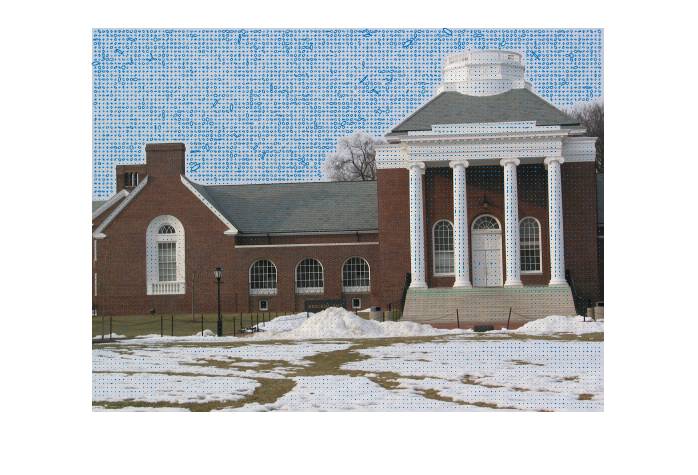
\includegraphics[scale=0.7]{I1w3.png}
\caption{Figure I1 with window size $w = 3$}
\label{I1w3}
\end{figure}
\begin{figure}[H]
\centering
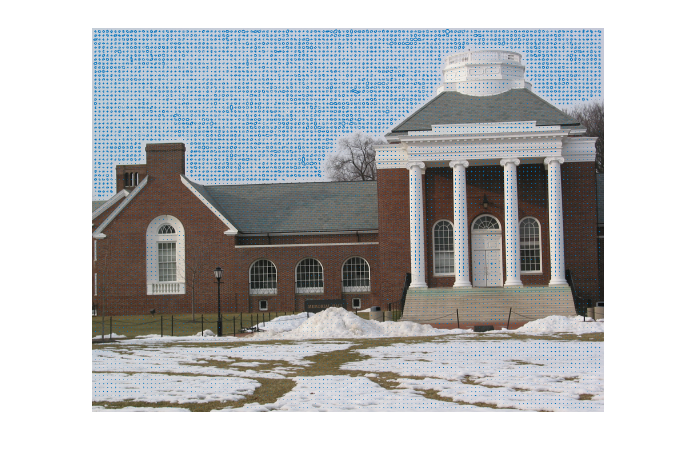
\includegraphics[scale=0.7]{I1w4.png}
\caption{Figure I1 with window size $w = 4$}
\label{I1w4}
\end{figure}
\begin{figure}[H]
\centering
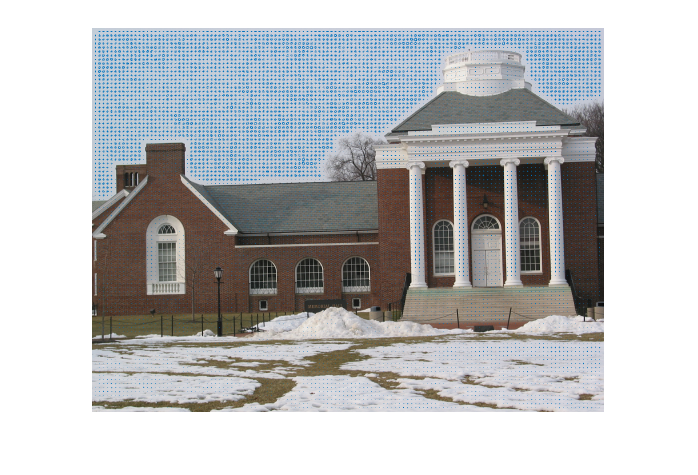
\includegraphics[scale=0.7]{I1w7.png}
\caption{Figure I1 with window size $w = 7$}
\label{I1w7}
\end{figure}
\begin{figure}[H]
\centering
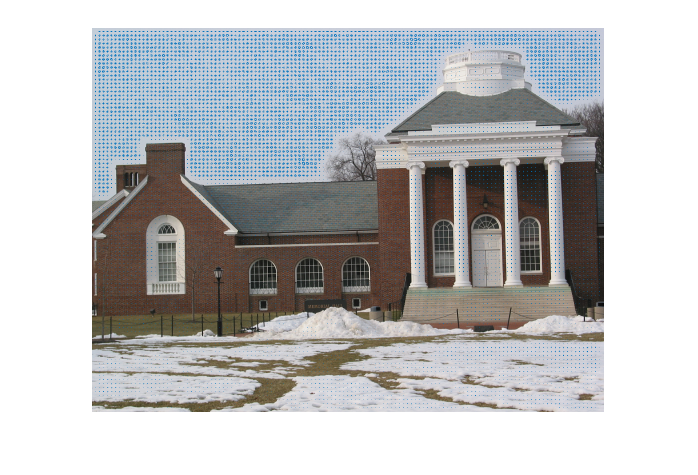
\includegraphics[scale=0.7]{I1w10.png}
\caption{Figure I1 with window size $w = 10$}
\label{I1w10}
\end{figure}
\begin{figure}[H]
\centering
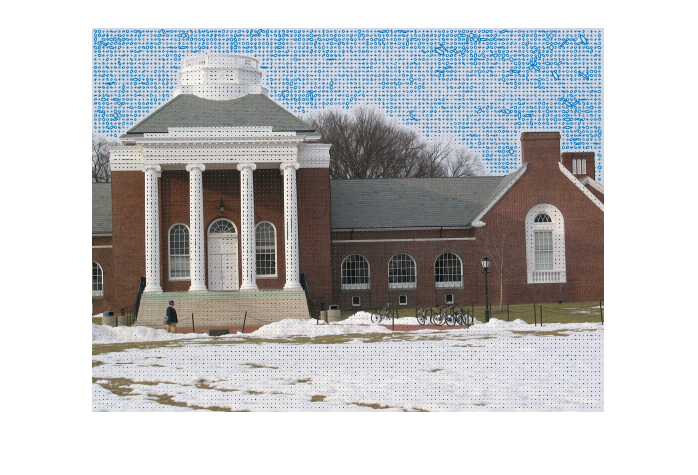
\includegraphics[scale=0.7]{I3w3.png}
\caption{Figure I3 with window size $w = 3$}
\label{I3w3}
\end{figure}
\begin{figure}[H]
\centering
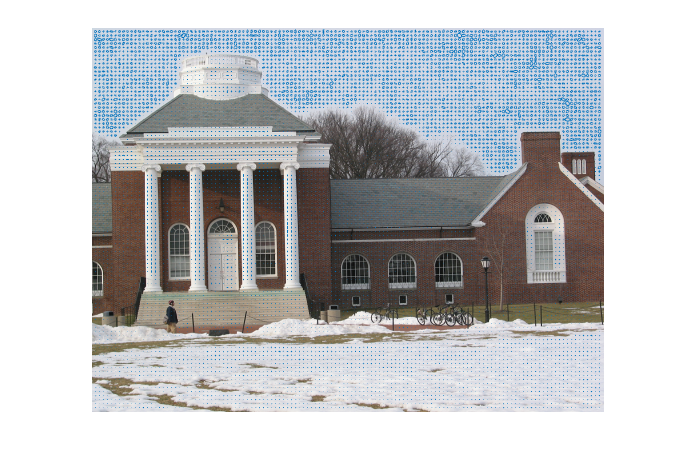
\includegraphics[scale=0.7]{I3w4.png}
\caption{Figure I3 with window size $w = 4$}
\label{I3w4}
\end{figure}
\begin{figure}[H]
\centering
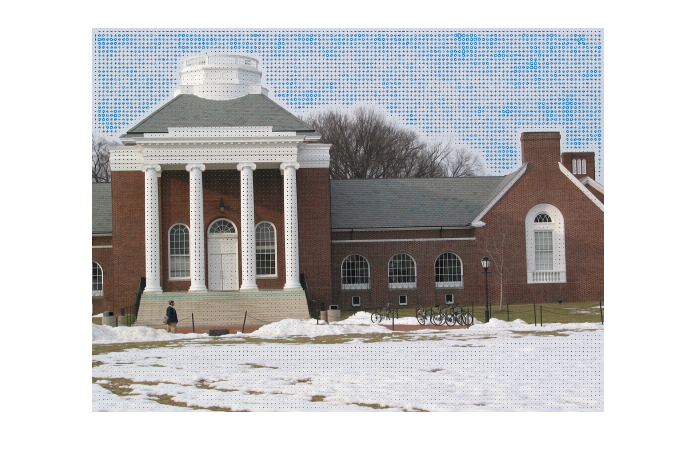
\includegraphics[scale=0.7]{I3w7.png}
\caption{Figure I3 with window size $w = 7$}
\label{I3w7}
\end{figure}
\begin{figure}[H]
\centering
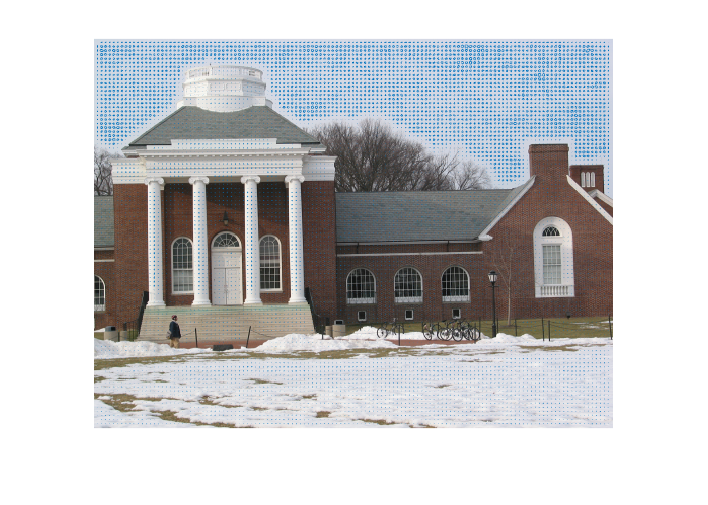
\includegraphics[scale=0.7]{I3w10.png}
\caption{Figure I3 with window size $w = 10$}
\label{I3w10}
\end{figure}

\subsection*{(c)}
The thresholds are chosen as $T = tR_{max}$ , where $R_{max}$ is defined as the maxinum corner response and takes value of $9.4191 \times 10^9$ for $I1.png$, and $1.0751 \times 10^{10}$ for $I3.png$. Take $t = 0.001$, $0.01$, $0.05$ and $0.1$. We show results for different t in Fig. \ref{tr1} $\sim$ \ref{rt8}. From the figure, we can see that while $T = 0.01 R_{max}$ captures a reasonable result, $T = 0.001R_{max}$ results including a lot of edge points besides corner points, indicating this threshold is too low. Also, $T = 0.1R_{max}$ and $T = 0.05R_{max}$ tends to lose some corner points, which is more apparently in the former case, indicating the threshold is too high.
\begin{figure}[H]
\centering
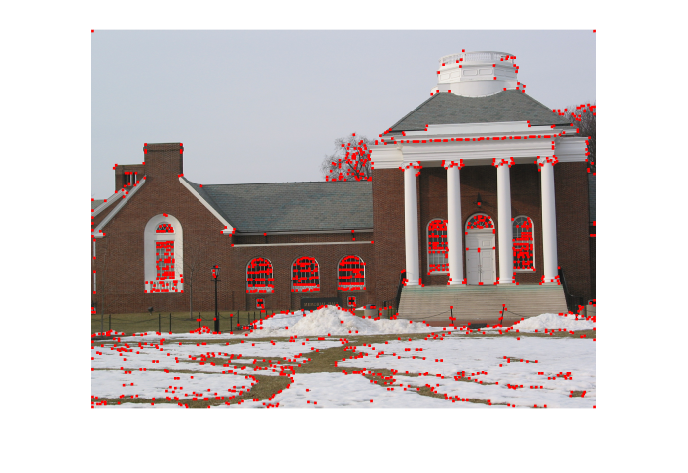
\includegraphics[scale=0.7]{I1t0001.png}
\caption{Harris Corner Detection with threshold $t = 0.001$}
\label{tr1}
\end{figure}
\begin{figure}[H]
\centering
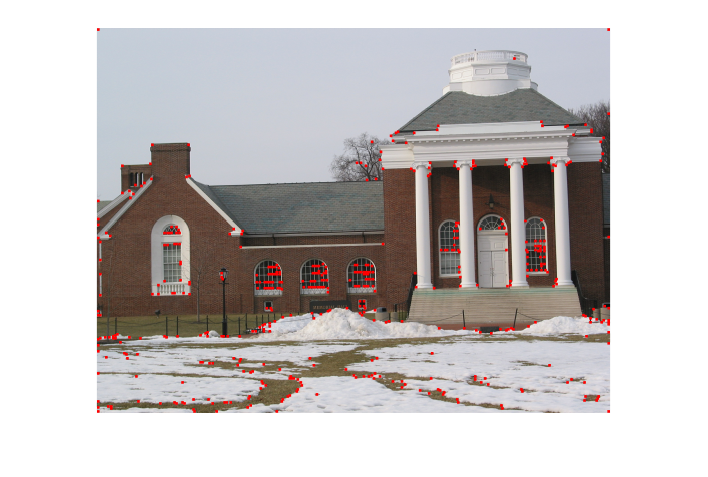
\includegraphics[scale=0.7]{I1t001.png}
\caption{Harris Corner Detection with threshold $t = 0.01$}
\label{tr2}
\end{figure}
\begin{figure}[H]
\centering
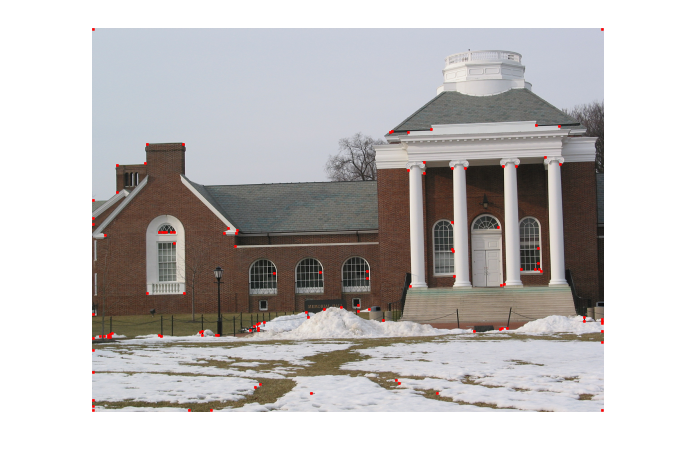
\includegraphics[scale=0.7]{I1t005.png}
\caption{Harris Corner Detection with threshold $t = 0.05$}
\label{tr3}
\end{figure}
\begin{figure}[H]
\centering
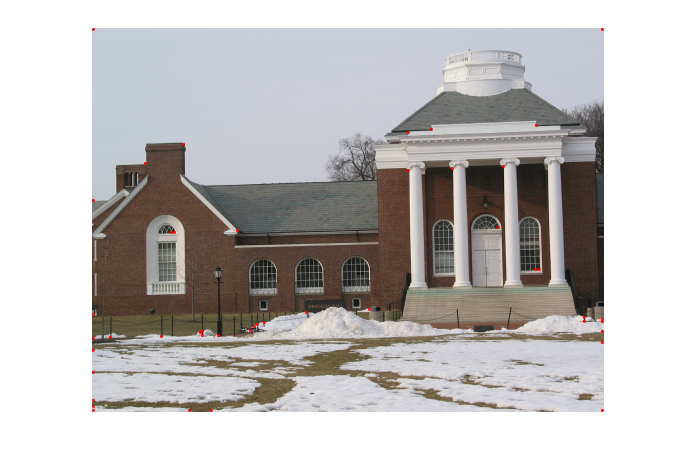
\includegraphics[scale=0.7]{I1t01.png}
\caption{Harris Corner Detection with threshold $t = 0.1$}
\label{tr4}
\end{figure}
\begin{figure}[H]
\centering
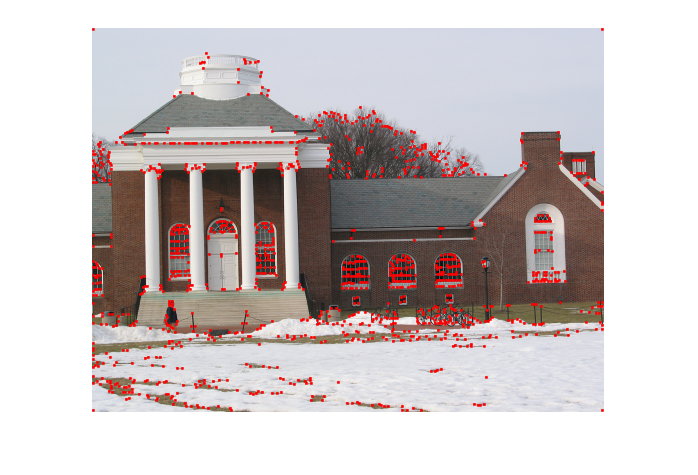
\includegraphics[scale=0.7]{I3t0001.png}
\caption{Harris Corner Detection with threshold $t = 0.001$}
\label{rt5}
\end{figure}
\begin{figure}[H]
\centering
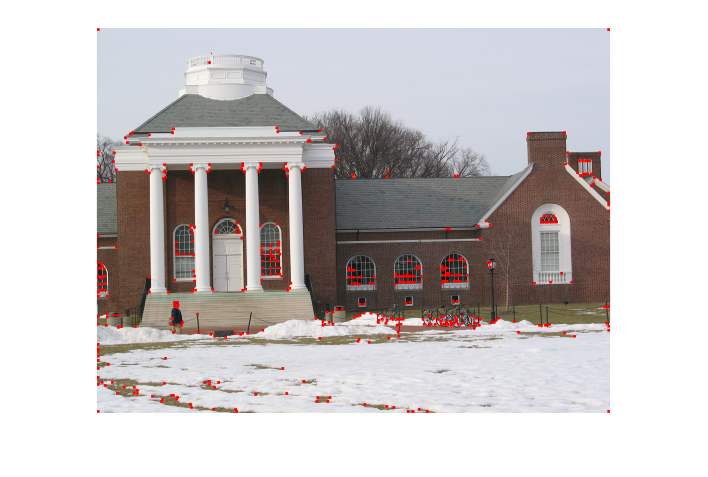
\includegraphics[scale=0.7]{I3t001.png}
\caption{Harris Corner Detection with threshold $t = 0.01$}
\label{rt6}
\end{figure}
\begin{figure}[H]
\centering
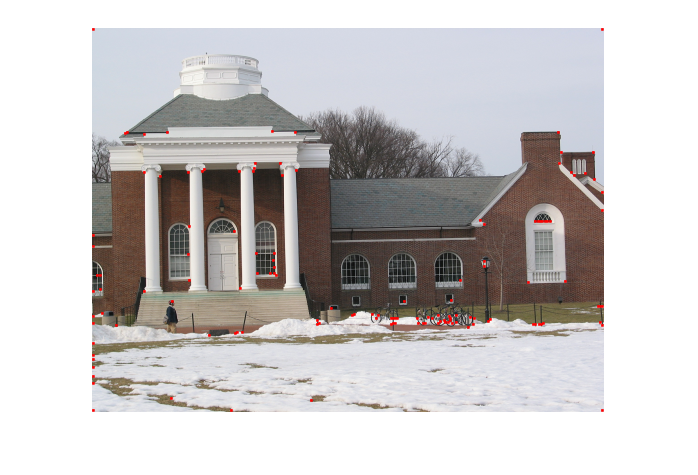
\includegraphics[scale=0.7]{I3t005.png}
\caption{Harris Corner Detection with threshold $t = 0.05$}
\label{rt7}
\end{figure}
\begin{figure}[H]
\centering
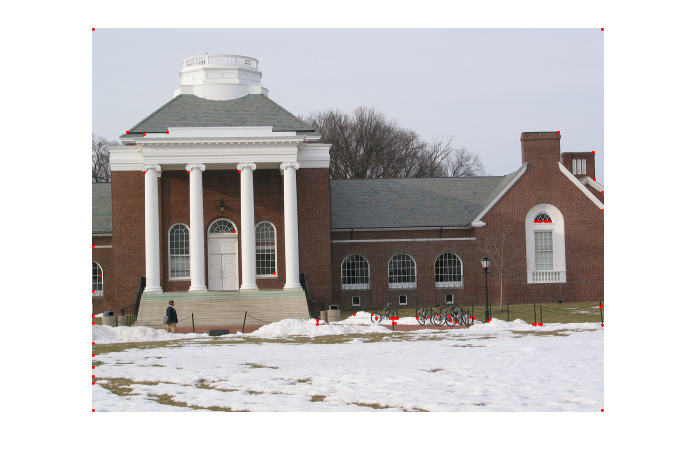
\includegraphics[scale=0.7]{I3t01.png}
\caption{Harris Corner Detection with threshold $t = 0.1$}
\label{rt8}
\end{figure}

\clearpage

\section*{Problem 2 \underline{Blob Detection}}
\subsection*{(a)}
The threshold is defined as $T = t\cdot R_{max}$, $R_{max}$ is the maximum value of scale space representation and $R_{max} = 1.1669\times 10^4$. When we take values of $t$ as 0.1, 0.2, 0.3 and 0.4, we will get results shown in the following figures. From Fig. \ref{q21}$\sim$\ref{q24}, it can be deduced that as we increase the threshold for Blob detection, the number of blob features we can detect will decrease. This is reasonable since a high threshold will neglect some less important features in the figure. The Matlab codes and detailed steps are attached behind.
\begin{figure}[H]
\centering
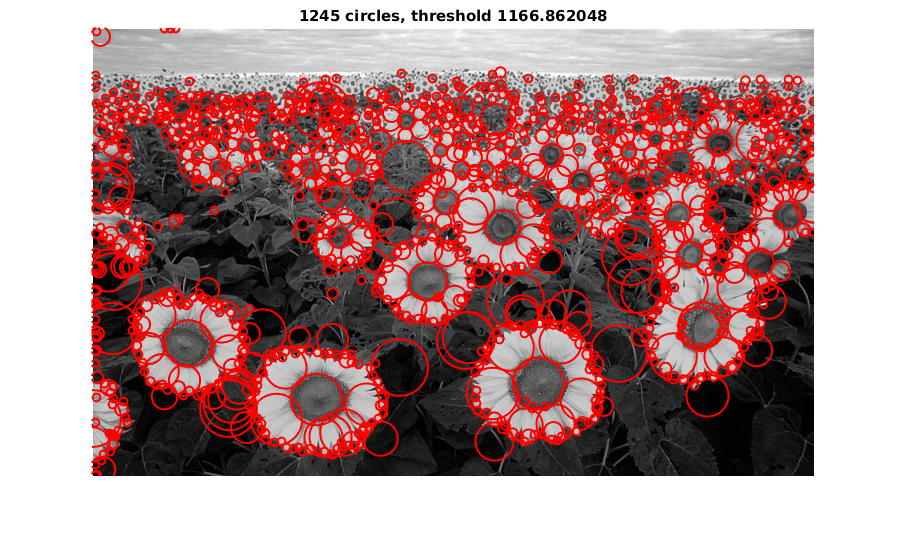
\includegraphics[scale=0.6]{q2t01.png}
\caption{Blob Detection with thresholds $t = 0.1$}
\label{q21}
\end{figure}
\begin{figure}[H]
\centering
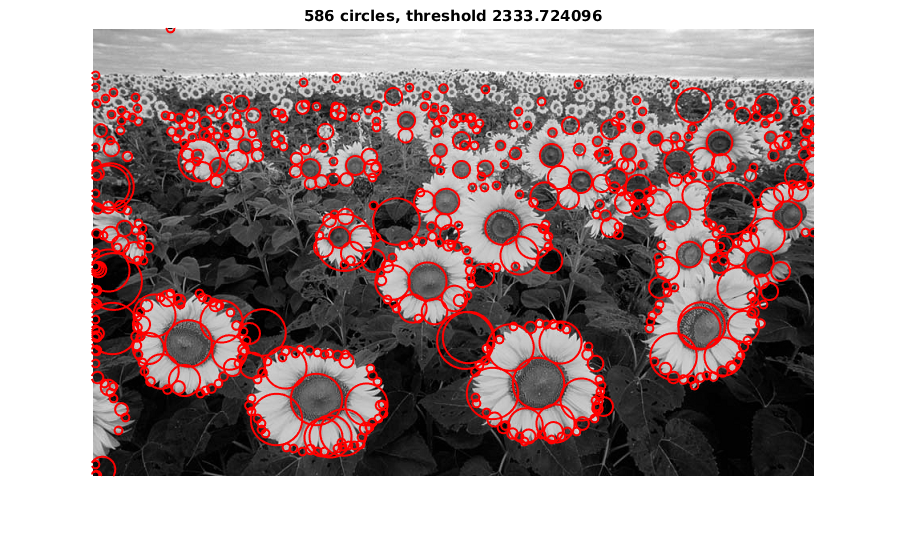
\includegraphics[scale=0.6]{q2t02.png}
\caption{Blob Detection with thresholds $t = 0.2$}
\label{q22}
\end{figure}
\begin{figure}[H]
\centering
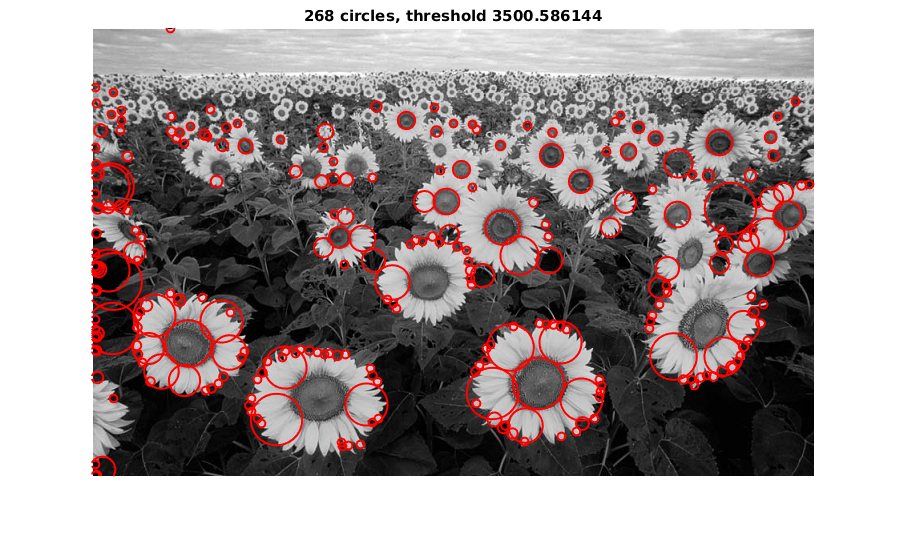
\includegraphics[scale=0.6]{q2t03.png}
\caption{Blob Detection with thresholds $t = 0.3$}
\label{q23}
\end{figure}
\begin{figure}[H]
\centering
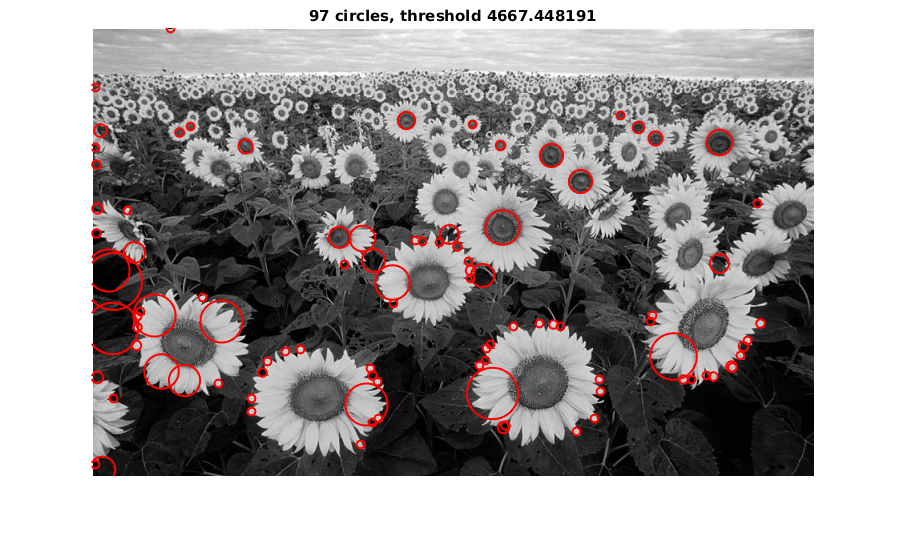
\includegraphics[scale=0.6]{q2t04.png}
\caption{Blob Detection with thresholds $t = 0.4$}
\label{q24}
\end{figure}
\subsection*{(b)}
The histogram is shown in Fig. \ref{q25}.
\begin{figure}[H]
\centering
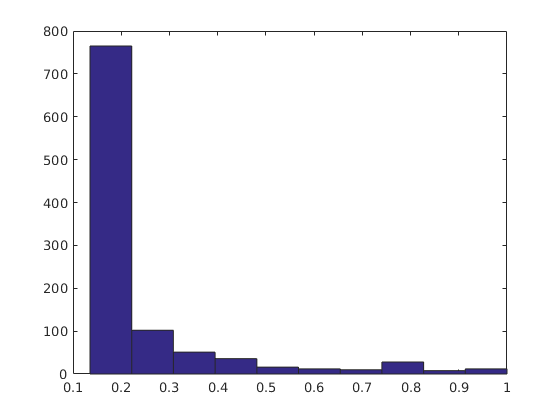
\includegraphics[scale=0.8]{q21500.png}
\caption{Relations between number of blobs and normalized blobs' radii in Blob Detection with thresholds $T = 1500$}
\label{q25}
\end{figure}
\lstinputlisting[firstline=1, lastline=200]{q2solution.m}


\end{document}